\begin{enumerate}[label=\thesubsection.\arabic*,ref=\thesubsection.\theenumi,itemsep=1pt]
 \item In an AP, if d=2, n=5 and $a_n=0$, then value of a is
    \begin{enumerate}
         \item 10
         \item 5
         \item -8
         \item 8
    \end{enumerate}
    \hfill (10, 2011) \item Find whether -150 is a term of the AP 17, 12, 7, 2,....?
    \hfill (10, 2011) \item Find the value of the middle term of the following AP :\[- 6, -2, 2,........, 58.\]
   \hfill (10, 2011) \item Determine the AP whose fourth term is 18 and the difference of the ninth term from the fifteenth term is 30.
\hfill (10, 2011) \item Find how many two-digit numbers are divisible by $6$.
 How many multiples of $4$ lie between $10$ and $250$ ? Also find their sum.
    \hfill (10, 2011)
         \item The ratio of the $11$\textsuperscript{th} term to $17$\textsuperscript{th} term of an A.P. is $3:4$. Find the ratio of $5$\textsuperscript{th} to $21$\textsuperscript{th} of the same A.P. Also, find the ratio of the sum of first $5$ terms to that of first $21$ terms
        \hfill (10, 2023) \item $250$ logs are stacked in the following manner:
        $22$ logs in the bottom row , $21$ in the next row, $20$ in the row next to it and so on. In how many rows are the $250$ logs placed and how many logs are there in top row ?
\hfill (10, 2023)
 \item If $-\frac{5}{7}$, $a$, $2$ are consecutive terms in an Arthimetic Progression, then the value of $a$ is 
    \begin{enumerate}
\item $\frac{9}{7}$
 \item $\frac{9}{14}$
 \item $\frac{19}{7}$
 \item $\frac{19}{14}$
    \end{enumerate}
    \hfill (10, 2022) \item Find the sum of first $16$ terms of an Arithmetic Progression whose $4^{\text{th}}$ and $9^{\text{th}}$ terms are $-15$ and $-30$ respectively.
    
        \hfill (10, 2022) \item If the sum of first $14$ terms of an Arithmetic Progression is $1050$ and its fourth term is $40$, find its $20^{\text{th}}$ term.

     \item 
    \begin{enumerate}
         \item Find the sum of the first twelve $2$-digit numbers which are 
multiples of $6$.

         \item In an AP, if $a_2=26$ and $a _ {15} = -26$, then write the AP.
        \end{enumerate}
         \item In Mathematics, relations can be expressed in various ways. The 
matchstick patterns are based on linear relations. Different strategies 
can be used to calculate the number of matchsticks used in different 
		\figref{fig:ap} 
 \\One such pattern is shown below. Observe the pattern and answer the 
following questions using Arithmetic Progression :
\begin{figure}[H]
    \centering
	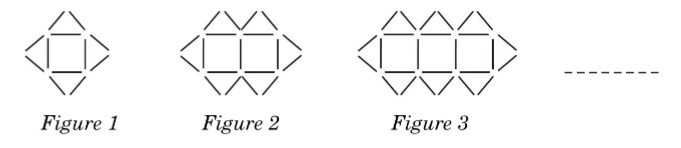
\includegraphics[width=\columnwidth]{figs/ap/ap.jpg}
	\caption{patterns of Figure1, figure2 ,figure3}
    \label{fig:ap}
\end{figure}
    \begin{enumerate}
	 \item Write the AP for the number of triangles used in the \figref{fig:ap}. Also, 
write the nth term of this AP.
 \item Which figure has $61$ matchsticks ? 
    \end{enumerate} 

    \hfill (10, 2022) 
 \item In an A.P. if the sum of third and seventh term is zero, find its $5^{\text{th}}$ term.
        \hfill (10, 2022)
  \item Determine the AP whose third term is $5$ and seventh term is $9$.
        \hfill (10, 2022) \item Find the sum of the first $20$ terms of an A.P. whose $n^{\text{th}}$ term is given as $a_n=5-2n$
        \hfill (10, 2022) \item Find the common difference 'd' of an AP whose first term is $10$ and the sum of the first $14$ terms is $1505$.

        \hfill (10, 2022) \item For what value of 'n', are the $n^{\text{th}}$ terms of the APs: $9,7,5,\dots$ and $15,12,9,\dots$ the same?
    \hfill (10, 2022)
\end{enumerate}
